\documentclass{article}
\usepackage{graphicx} % Required for inserting images
\usepackage{hyperref} 

\title{Introducción a Packet Tracer}
\author{Diego Cono}
\date{Agosto 2024}

\begin{document}

\maketitle

\section{Packet Tracer}
    \subsection{Herramientas Básicas}

        Las herramientas básicas de Packet Tracer son componentes esenciales que permiten construir, configurar y simular una red. Estas herramientas incluyen dispositivos de red que gestionan el tráfico entre distintas partes de la red, dispositivos de usuario que representan las computadoras y otros equipos conectados a la red, y cables y conexiones que permiten la comunicación entre estos dispositivos.  

    \subsection{Modos de Operación}
        Los modos de operación en Packet Tracer son diferentes formas en las que puedes interactuar y trabajar con la red simulada. Cada modo ofrece una perspectiva o funcionalidad distinta:
        \begin{itemize}
            \item Modo Tiempo Real: Permite observar cómo funciona la red como lo haría en un entorno real, con dispositivos operando en tiempo real.
            \item Modo Simulación: Facilita el análisis detallado del tráfico de la red al ralentizar la comunicación, permitiendo ver el paso a paso de cómo se transmiten los datos.
            \item Modo de Configuración: Te permite configurar y ajustar los dispositivos en la red, personalizando su comportamiento y funciones.
            \item Modo de Prueba: Permite verificar y validar la configuración y conectividad de la red mediante pruebas y comandos específicos.
        \end{itemize}
        
\section{Dispositivos Finales}
    Los dispositivos finales en Packet Tracer que incluyen PCs, Laptops, Servidores e Impresoras son componentes esenciales que representan los puntos de interacción directa en una red:
    \begin{itemize}
        \item PCs (Computadoras Personales): Son estaciones de trabajo que se conectan a la red para acceder a recursos y servicios, permitiendo la comunicación entre usuarios y otros dispositivos.
        \item Laptops: Similares a las PCs, pero con la capacidad de conectarse tanto a redes cableadas como inalámbricas, ofreciendo movilidad dentro de la red.
        \item Impresoras: Dispositivos de salida que permiten a los usuarios imprimir documentos y otros archivos, conectándose a la red para recibir trabajos de impresión desde diferentes dispositivos.
        \item Servidores: Dispositivos que proporcionan servicios y recursos a otros dispositivos en la red, como almacenamiento de datos, aplicaciones, o servicios web.
    \end{itemize}
    
\section{Dispositivos de Red}
    Los dispositivos de red en Packet Tracer, como routers, switches y hubs, son fundamentales para gestionar la comunicación en una red:
    \begin{itemize}
        \item Routers: Dispositivos que dirigen el tráfico de datos entre diferentes redes, determinando la mejor ruta para cada paquete de datos.
        \item Switches: Dispositivos que conectan múltiples dispositivos dentro de una misma red local, gestionando el tráfico de datos de manera eficiente para asegurarse de que los paquetes lleguen al destino correcto.
        \item Hubs: Dispositivos que conectan varios dispositivos en una red, retransmitiendo los datos recibidos a todos los puertos conectados, sin diferenciar el destino.
    \end{itemize}
        
\section{Cableado}
    El cableado en Packet Tracer incluye diversos tipos de cables que facilitan la conexión y comunicación entre dispositivos:
        \begin{itemize}
            \item Cable de Consola: Utilizado para la configuración inicial y gestión de dispositivos de red a través de una conexión directa.
            \item Cable USB: Utilizado para conectar dispositivos a una computadora para configuración o transferencia de datos, ofreciendo una conexión rápida y directa.
            \item Cable Straight Through: Conecta dispositivos de diferentes tipos, como computadoras y switches, transmitiendo señales en línea recta.
            \item Cable Cross Over: Conecta dispositivos del mismo tipo, como dos computadoras o dos switches, cruzando las señales para la comunicación directa entre ellos.
            \item Fibra Óptica: Utilizado para conexiones de alta velocidad a largas distancias, transmitiendo datos mediante pulsos de luz.
        \end{itemize}
\section{Actividad}
    Se interconectarán dos PCs vía una simple conexión cruzada, observando los elementos necesarios:
    
    \begin{figure}[h]
        \centering
        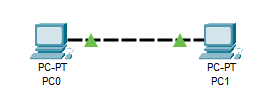
\includegraphics[width=0.5\linewidth]{pcs.png}
    \end{figure}
    El problema de esta conexión directa, es decir, sin usar dispositivos de red, es que no podemos agregar más computadoras a la red.
\section{Referencias}
    \href{https://github.com/diego-g-cono/diego-g-cono/blob/master/cono.tex}{cono.tex}
\end{document}
